\documentclass{beamer}
\usetheme{Warsaw}

\usepackage[utf8]{inputenc}
\usepackage{fancybox}
\usepackage{multimedia} 
\usepackage{subfig}
\usepackage{amsmath}
\usepackage{hyperref}
\usepackage[all]{xy}
\begin{document}


\title[Stochastik] % (optional, only for long titles)
{Stochastik für Informatiker
\\
\includegraphics[scale=0.5]{img/craps}
}
\subtitle{}
\author[Dr. Johannes Riesterer] % (optional, for multiple authors)
{Dr.  rer. nat. Johannes Riesterer}

\date[KPT 2004] % (optional)
{}

\subject{Stochastik}

\frame{\titlepage}

\begin{frame}
    \frametitle{Allgemeine Wahrscheinlichkeitsräume}
\framesubtitle{}
\begin{block}{Maßraum}
Ein Maßraum ist ein Tripel $(\Omega, \mathcal{A}, \mu)$ bestehend aus der Grundmenge $\Omega$, einer $\sigma$-Algebra $\mathcal{A} \subset  \mathcal{P}(\Omega)$ und einer Abbildung

\begin{align*}
& \mu : \mathcal{A} \to [0,\infty] \\
& \mu (\emptyset)  = 0 \\
 & \;  \mu \biggl(  \bigcup_i A_i  \biggr) = \sum_i \mu(A_i), \text{ mit } A_i \cap A_j = \emptyset \text{ für } i \neq j
\end{align*}
Mengen mit $\mu(M) = 0$ werden Nullmengen genannt.
\end{block}
 \end{frame}


\begin{frame}
    \frametitle{Allgemeine Wahrscheinlichkeitsräume}
\framesubtitle{}
\begin{block}{Messbare  Abbildung}
Ein Abbildung  $f : \Omega \to R$ zwischen einem Maßraum  $(\Omega, \mathcal{A}, \mu)$  und einer $\sigma$-Algebra $(R,  \mathcal{B} )$ heißt messbar, falls 
\begin{align*}
f^{-1}(B) \in \mathcal{A} \text{ für alle } B \in  \mathcal{B}
\end{align*}
gilt. (Urbilder von Messbaren Mengen sind Messbar).

Für eine messbare Funktion  $f: \Omega \to \mathbb{R}$ existiert eine endliche Reihe 
\begin{align*}
& s_n(x) := \sum_{i = 1}^{n} c_i \cdot 1_{A_j} \\
 & s_n(x) \leq f(x) \\
 & \lim_{n \to \infty}  s_n(x) \to f(x)  \text{ für alle x  } \in \Omega
\end{align*}
Man nennt $s_n$ auch einfache Funktion. \end{block}
 \end{frame}

\begin{frame}
    \frametitle{Inegration}
\framesubtitle{}

\begin{block}{Integration}
Für eine einfache Funktion   $s_n : \Omega \to \mathbb{R}$  definiere
\begin{align*}
\int_\Omega s_n(x) \;  d\mu := \sum_{i=1}^{n} c_i \; \mu(A_i)
\end{align*}
\end{block}
\begin{block}{Maßraum}

Für eine positive Funktion $f: \Omega \to [0, \infty]$ definiere

\begin{align*}
\int_\Omega f(x) \;  d \mu = \sup( \int_\Omega s_n(x) \;  d\mu ; s_n(x) \text{ einfach mit } s_n(x) \leq f(x))
\end{align*}
\end{block}
 \end{frame}



\begin{frame}
    \frametitle{Integration}
\framesubtitle{}

\begin{block}{Integration}
Für allgemeines $f$ zerlege $f = f^+ - f^-$ mit $f^+ := \max(0, f)$ und $f^- := -min(0, f)$ und definiere 
\begin{align*}
\int_\Omega f(x) \;  d\mu  = \int_\Omega f^+(x) \;  d\mu - \int_\Omega f^-(x) \;  d\mu
\end{align*}

\end{block}


 \end{frame}


\begin{frame}
    \frametitle{Allgemeine Wahrscheinlichkeitsräume}
\framesubtitle{}
\begin{block}{Wahrscheinlichkeitsdichte}
Eine messbare Funktion $f: \Omega  \to \mathbb{R}$ mit $\int_{\Omega} f(x) \; d\mu = 1$ heißt Dichte.
\end{block}
\begin{block}{Wahrscheinlichkeitsmaß}
Ist $f: \Omega  \to \mathbb{R}$ eine Dichte, so definiert 
\begin{align*}
P_f (A) := \int_{A} f (x) dx
\end{align*}
 ein Wahrscheinlichkeitsmaß auf $\mathcal{A}$.
\end{block}
 \end{frame}


\begin{frame}
    \frametitle{Allgemeine Wahrscheinlichkeitsräume}
\framesubtitle{}
\begin{block}{Beispiel (Normalverteilung)}
$\Omega = R = \mathbb{R}$ mit Borell'scher Sigma-Algebra. 
$ f(x) = \frac 1{\sigma \sqrt{2\pi}}e^{- \frac {1}{2} (\frac{x- \mu}{ \sigma})^2}$ mit $\mu \in \mathbb{R}, \sigma > 0 $.
\begin{align*}
P_f (A) := \int_{A}  \frac 1{\sigma \sqrt{2\pi}}e^{- \frac {1}{2} (\frac{x- \mu}{ \sigma})^2}dx
\end{align*}

\end{block}

\begin{figure}[htp]
      \centering
    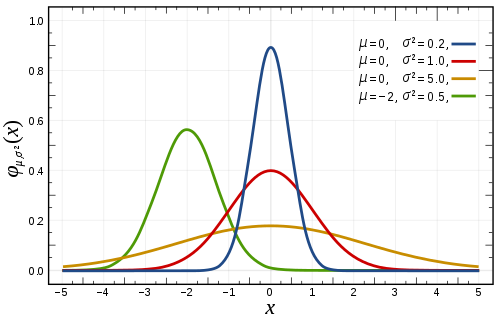
\includegraphics[width=0.55\textwidth]{img/normal}
      \caption{Quelle: Wikipedia}
\end{figure}


 \end{frame}

\begin{frame}
    \frametitle{Allgemeine Wahrscheinlichkeitsräume}
\framesubtitle{}
\begin{block}{Beispiel (Normalverteilung)}
\begin{align*}
& I := \int_{0}^{\infty} e^{-x^2} \; dx\\
& I^2 = \int_{0}^{\infty} \int_{0}^{\infty} e^{-(x^2+y^2)} \; dx \;dy \\
&x=r \cos \varphi ,y=r\sin \varphi ,r^2 = x^2 + y^2  \; (\text{ da } \cos^2 + \sin^2 = 1)\\
 &\text{ \href{https://de.wikipedia.org/wiki/Polarkoordinaten\#Zylinderkoordinaten}{LINK: Polarkoordinatentransformation}} \\
& = \int_{0}^{\frac{\pi}{2}}  \int_{0}^{\infty}r \cdot e^{-r^2} \; dr \;d\varphi \\
&= \frac{\pi}{2} \int_{0}^{\infty}r \cdot e^{-r^2} \; dr \\
&= -\frac{\pi}{4} [e^{-r^2} ]_0^{\infty} = \frac{\pi}{4} \Rightarrow I = \frac{\sqrt{\pi}}{2}
\end{align*}
\end{block}



 \end{frame}




\begin{frame}
    \frametitle{Allgemeine Wahrscheinlichkeitsräume}
\framesubtitle{}
\begin{block}{Bildmaß}
Ist $X : \Omega \to R$  eine Zufallsvariable zwischen einem Wahrscheinlichkeitsraum  $(\Omega, \mathcal{A}, P)$  und einer $\sigma$-Algebra $(R,  \mathcal{B} )$, so definiert 
\begin{align*}
P_X(B) := P(X^{-1}(B))
\end{align*}
ein Wahrscheinlichkeitsmaß auf $(R, \mathcal{B})$. Ist  $R = \mathbb{R}$, so nennen wir  $X$ eine reelle Zufallsvariable. Ist $\Omega$ albzählbar, so heißt $X$ diskrete Zufallsvariable.
\end{block}

 \end{frame}

\begin{frame}
    \frametitle{Allgemeine Wahrscheinlichkeitsräume}
\framesubtitle{}
\begin{block}{Beispiel (Summe zweier Würfel)}
$\Omega = \{1,2,3,4,5,6 \} \times \{1,2,3,4,5,6 \} $, $R = \{ 2,3,4,5,6,7,8,9,10, 11, 12\}$ und $X: \Omega \to R; X (a,b) := a +b$. Dann ist 
$P_X(3) = P((1,2), (2,1)) = \frac{2}{36} = \frac{1}{18}$ 
\end{block}

 \end{frame}

\begin{frame}
    \frametitle{Allgemeine Wahrscheinlichkeitsräume}
\framesubtitle{}
\begin{block}{Bedingte Wahrscheinlichkeit}
Ist   $(\Omega, \mathcal{A}, P)$ ein Wahrscheinlichkeitsraum und $A,B \in \mathcal{A}$ mit $P(B)>0$, so heißt
\begin{align*}
P(A | B) := \frac{P(A \cap B)}{P(B)}
\end{align*}
die bedingte Wahrscheinlichkeit von $A$ unter (der Hypothese) $B$.
\end{block}
\begin{block}{Stochastische unabhängigkeit}
Zwei Ereignisse $A,B \in \mathcal{A}$ heißen stochastisch unabhängig, falls 
\begin{align*}
P(A \cap B) = P(A) \cdot P(B)
\end{align*}
gilt. Ist  $P(B)>0$, so folgt $P(A | B) = P(A)$.
\end{block}

 \end{frame}


\begin{frame}
    \frametitle{Allgemeine Wahrscheinlichkeitsräume}
\framesubtitle{}
\begin{block}{Erwartungswert}
Ist $X : \Omega \to \mathbb{R}$  eine reelle Zufallsvariable, so ist Ihr Erwartungswert definiert durch
\begin{align*}
\mathbb{E}(X) := \int_\Omega X \; d\mu \; \; ( \text{kontinuierlich})  \\
\mathbb{E}(X) := \sum_{x} X(x) P(x) \; \; ( \text{diskret}) 
\end{align*}
\end{block}
\begin{block}{Eigenschaften}
Sind $X,Y : \Omega \to \mathbb{R}$   reelle Zufallsvariablen und $a,b \in \mathbb{R}$ konstant, so gilt:
\begin{align*}
\mathbb{E}(a \cdot X + b \cdot Y) = a \cdot \mathbb{E}(X) + b \cdot \mathbb{E}(Y) 
\end{align*}
\end{block}

 \end{frame}

\begin{frame}
    \frametitle{Allgemeine Wahrscheinlichkeitsräume}
\framesubtitle{}
\begin{block}{Erwartungswert Beispiele}
$\Omega = R = \mathbb{R}$ mit Borell'scher Sigma-Algebra, $X(x) = x$ und
\begin{align*}
P_f (A) := \int_{A}  \frac 1{\sigma \sqrt{2\pi}}e^{- \frac {1}{2 } (\frac{x- \mu}{ \sigma})^2}dx
\end{align*}
Dann ist 
\begin{align*}
\mathbb{E}(X) & := \int_{\mathbb{R}}  x \cdot  \frac 1{\sigma \sqrt{2\pi}}e^{- \frac {1}{2 } (\frac{x- \mu}{ \sigma})^2} \; dx  \\
&= \int_{\mathbb{R}}  (y + \mu) \cdot  \frac 1{\sigma \sqrt{2\pi}}e^{- \frac {1}{2 \sigma^2} y^2} \; dy \\
 &  = \mu  \int_{\mathbb{R}}      \frac 1{\sigma \sqrt{2\pi}}e^{- \frac {1}{2 \sigma^2} y^2} \; dy  + \int_{\mathbb{R}}  y  \cdot  \frac 1{\sigma \sqrt{2\pi}}e^{- \frac {1}{2 \sigma^2} y^2} \; dy = \mu
\end{align*}
\end{block}
 \end{frame}

\begin{frame}
    \frametitle{Allgemeine Wahrscheinlichkeitsräume}
\framesubtitle{}
\begin{block}{Erwartungswert Beispiele}
$\Omega = \{ \text{Kopf},\text{Zahl}\}$, $P(\text{Kopf}) = P(\text{Zahl}) = \frac{1}{2}$, $X(\text{Kopf}) = 0,  X(\text{Zahl}) = 1$ 
\begin{align*}
& \mathbb{E}(X)  = 0 \cdot P(X^{-1}(0) ) + 1 \cdot P(X^{-1}(1)) \\
& =0  \cdot P(\text{Kopf}) + 1 \cdot P(\text{Zahl}) = \frac{1}{2}  
\end{align*}
\end{block}

 \end{frame}

\begin{frame}
    \frametitle{Allgemeine Wahrscheinlichkeitsräume}
\framesubtitle{}

\begin{block}{Varianz}
Die Varianz ist definiert durch
\begin{align*}
\mathbb{V}(X) :=\mathbb{E}( (X - \mathbb{E}(X)^2 )
\end{align*}
\end{block}

 \end{frame}


\end{document}
